\documentclass[aspectratio=169,usenames,dvipsnames]{beamer}
\usepackage{preamble}
\title{Coding for Humanities, week 3}

\begin{document}

\begin{frame}
 \titlepage
\end{frame}

\begin{frame}{Plan for today}
 \tableofcontents
\end{frame}

\begin{frame}{Motivation}
    Until now:
    \begin{itemize}
        \item Work with simple values (numbers, text)
        \item Create complex values (lists, dictionaries)
        \item Store results in memory (variables)
    \end{itemize}

    \pause
    What's missing:
    \begin{itemize}
        \item Making decisions
        \item Repetition
    \end{itemize}
\end{frame}

\begin{frame}{Making decisions: flow charts}
    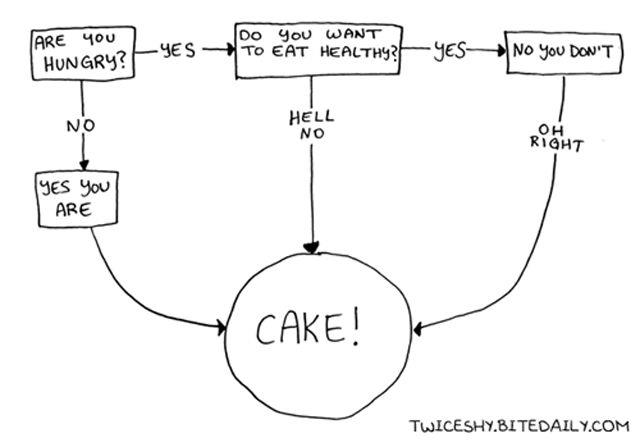
\includegraphics[height=0.8\textheight]{fig/flowchart}
\end{frame}

\section{Conditional statements: do you really want to do that?}
\frame{\tableofcontents[currentsection]}

\begin{frame}{Simple conditions}
    \begin{definition}
        A \structure{conditional expression} is
        an expression that is \texttt{True} or \texttt{False}
    \end{definition}
    \begin{description}
        \item[a == b] are the values equal?
        \item[a != b] inequality
        \item[a $<$ b] test whether a is smaller than b
        \item[a $>$ b]
        \item[a in b] does element a occur in the sequence/dict b?
    \end{description}

    NB: == tests equality, \\
        = is an assignment statement!
\end{frame}

\begin{frame}[fragile]{The if-statement}
\begin{lstlisting}
if books > 5:
    print('you are an avid reader')
\end{lstlisting}

    \begin{itemize}
        \item The code under an if-statement is only executed
            if the condition is True.
        \item The indentation determines which code is covered
            by the condition
    \end{itemize}

    \pause
    \begin{definition}
        A \structure{code block} is a sequence of indented lines after
        a statement ending in `:'.
        The start and end of the block are defined by the indentation of the
        lines.
    \end{definition}
\end{frame}


\begin{frame}[fragile]{Optional extensions of the if-statement}
\begin{lstlisting}
if books > 5:
    print('you are an avid reader')
else:
    print('you should read more')
\end{lstlisting}

\begin{itemize}
    \item The code under 'else' is executed if the condition does NOT match.
\end{itemize}
\end{frame}


\begin{frame}[fragile]{Optional extensions of the if-statement}
\begin{lstlisting}
if books > 5:
    print('you are an avid reader')
elif books > 15:
    print('you should get out more')
else:
    print('you should read more')
\end{lstlisting}

\begin{itemize}
    \item Can add multiple extra conditions with 'elif' (else if)
    \item The conditions are tested from top to bottom;
            when one of them matches, the rest are ignored.
\end{itemize}
\end{frame}


\begin{frame}{Complex conditions}
    Can create complex conditions from other conditions:
    
    \begin{description}
        \item[cond1 and cond2]
        \item[cond1 or cond2]
        \item[not cond]
    \end{description}

\end{frame}

\begin{frame}[fragile]{Truthy and Falsy things}
\begin{itemize}
\item The number zero and empty sequences are treated as False.
\item Nonzero numbers and nonempty sequences are treated as True
\end{itemize}

These are equivalent:
\begin{lstlisting}
if len(books) != 0:
    print('yes')    
if len(books):
    print('yes')    
if books:
    print('yes')    
\end{lstlisting}

\end{frame}

\begin{frame}[fragile]{Converting a decision tree into if-statements}
    \begin{columns}
        \column{0.5\linewidth}
            ``Should you stay at a social gathering?''

            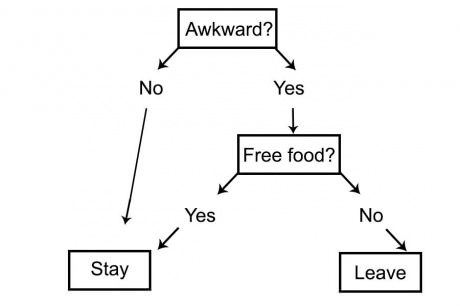
\includegraphics[width=0.8\textwidth]{fig/flowchart2}

        \pause
        \column{0.5\linewidth}
\begin{lstlisting}
awkward = False
free_food = True
if awkward:
    if free_food:
        print('Stay')
    else:
        print('Leave')
else:
    print('Stay')
\end{lstlisting}
\end{columns}
\end{frame}


\begin{frame}{Summary}
    \begin{description}
        \item[Conditions] An expression that is \texttt{True} or \texttt{False}.

                Comparisons, equality tests: <, >, ==, !=

                Complex conditions: \texttt{and, or, not}

        \item[if-statements] Execute statements only if condition is True
    \end{description}
\end{frame}


\section{Loops: play it again, Sam!}
\frame{\tableofcontents[currentsection]}

\begin{frame}[fragile]{Repeating statements: loops}
\begin{lstlisting}
books = ['a', 'b', 'c']
for book in books:
    print(book)
\end{lstlisting}
Result:
\begin{lstlisting}
a
b
c
\end{lstlisting}

\begin{itemize}
\item The statements under the for-loop are repeated
    for every element in the sequence.
\item At every iteration, 'book' contains an element of 'books'
\end{itemize}
\end{frame}

\begin{frame}[fragile]{Looping over sequences}
For loops can be used for anything with multiple items:
\begin{lstlisting}
for letter in 'word':
    print(letter)
for number in [0, 1, 2]:
    print(number)
\end{lstlisting}
\end{frame}

\begin{frame}[fragile]{Looping over dictionaries}
Looping over a dictionary returns only the keys:
\begin{lstlisting}
data = {'a': 0, 'b': 1}
for key in data:
    print(key)
    print(data[key])
\end{lstlisting}

\pause
Often want both the key and the value:
\begin{lstlisting}
for key, value in data.items():
    print(key)
    print(value)
\end{lstlisting}
\end{frame}


\begin{frame}[fragile]{Looping without a list}
Can use the \texttt{range} function if we don't have a list:
\begin{lstlisting}
for number in range(4)
    print(number)
\end{lstlisting}

Result:
\begin{lstlisting}
0
1
2
3
\end{lstlisting}

Repeats 4 times. Last item is 3 because counting starts at 0.
\end{frame}

\begin{frame}{Summary}
    \begin{description}
        \item[for-loop] repeat code for each element
        \item[iterables] strings, lists, dictionaries
        %\item[]
    \end{description}
\end{frame}

\end{document}
